\chapter{Results} \label{results}
    \blindtext
    
    \longsection{Impact of TOF on Respiratory Motion Modelling using NAC PET}{impact_of_tof_on_respiratory_motion_modelling_using_nac_pet}
        \gls{RM} reduces image quality in \gls{PET}. Unless gated \gls{CT} or \gls{MR} data are available, \gls{MC} relies on registration of the \gls{PET} data. To avoid mis-registration due to attenuation mismatches, most existing methods rely on pair wise registration of \gls{NAC} \gls{PET} volumes. This is a challenging problem due to the low contrast and high noise of these volumes. This section investigates the possibility of using \gls{MM}s for respiratory \gls{MC} in \gls{PET}, and in particular whether incorporating \gls{TOF} information increases the accuracy of the \gls{MM}s derived from the \gls{NAC} reconstructed images. \gls{XCAT} phantom simulations are used for $1$ bed position with a \gls{FOV} including the base of the lungs and the diaphragm. A \gls{TOF} resolution of $375$ picoseconds is used. \gls{NAC} images are reconstructed using \gls{OSEM} and used as input for \gls{MM} estimation. Different \gls{MM}s are compared using the original \gls{XCAT} input volumes. The results indicate that \gls{TOF} improves the accuracy of the \gls{MM} considerably.
        
        \subsection{Introduction} \label{impact_of_tof_on_respiratory_motion_modelling_using_nac_pet_introduction}
        \gls{RM} causes artefacts and loss of resolution in the thoracic region in \gls{PET}~\boxcite{Nehmeh2008}. Many methods have been proposed to correct for \gls{RM}, usually involving registration between a reference volume and a set of volumes in different positions in the respiratory cycle obtained by gating~\boxcite{Oliveira2014}. However, such pair wise registration is sensitive to noise. It also does not allow prediction of the respiratory state for data not used to estimate the motion, for instance, to be used for real time \gls{MC}. Surrogate driven \gls{MM}s attempt to overcome these deficiencies by relating the motion in the data to a number of \gls{SS}s~\boxcite{McClelland2013}. The model outputs a transformation or \gls{DF} for every value of the \gls{SS}s. \gls{MM}s are calculated on a series of either time or gating based volumes.

        The benefits of using \gls{AC} \gls{PET} for \gls{IR} are unclear. If images are reconstructed using a static \gls{mu-map}, then artefacts caused by the misalignment between the activity distribution and the \gls{mu-map} would hamper \gls{IR}. It could therefore be advantageous to estimate motion on \gls{NAC} images~\boxcite{WenjiaBai2011}. However, contrast may be too low to calculate an accurate \gls{MM} and artefacts associated with the mismatch between the acquisition and system model could also obscure the underlying motion. 
        
        In the absence of \gls{TOF}, there is no information on the activity position along the \gls{LOR} and \gls{NAC} reconstructions have high intensity near the surface and low contrast in the internal part of the body. In \gls{TOF}, the time information constrains the activity position along the \gls{LOR} changing the nature and extent of the artefacts associated with \gls{NAC} as well as changing noise properties~\boxcite{Ter-Pogossian1981}.
        
        The aim of this section is to investigate whether \gls{TOF} can sufficiently increase the contrast and lower the noise of \gls{NAC} images to facilitate the calculation of accurate \gls{MM}s.
        
        \subsection{Methods} \label{impact_of_tof_on_respiratory_motion_modelling_using_nac_pet_methods}
            \subsubsection{XCAT Image Generation} \label{impact_of_tof_on_respiratory_motion_modelling_using_nac_pet_methods_xcat_image_generation}
                \gls{XCAT}~\boxcite{Segars2010} was used to generate $6$ volumes over a linear $5$ second breathing cycle, with $1$ volume at full expiration at the beginning of the cycle and $1$ volume at full expiration at the end of the cycle and using settings for the extent of \gls{AP} and \gls{SI} motion. Activity concentrations were derived from a static \gls{FDG} patient scan. The \gls{FOV} included the base of the lungs, diaphragm and the top of the liver with a $40$ millimetre diameter spherical lesion placed in the right lung.
            
            \subsubsection{PET Data Simulation} \label{impact_of_tof_on_respiratory_motion_modelling_using_nac_pet_methods_pet_data_simulation}
                \gls{PET} acquisitions were simulated using \gls{STIR}~\boxcite{Thielemans2012},~\boxcite{Efthimiou2018} through \gls{SIRF}~\boxcite{ovtchinnikov2019SIRFSynergisticImage,ovtchinnikov_evgueni_2019_3548719} to forward project the input data to sinograms using the geometry of a GE Discovery 710 and, where relevant, a \gls{TOF} resolution of $375$ picoseconds similar to the GE Signa \gls{PET}/\gls{MR} (using \gls{TOF} mashing to reduce computation time resulting in $13$ \gls{TOF} time bins of size $376.5$ picoseconds). Attenuation was included in the simulation using the relevant \gls{mu-map} generated by \gls{XCAT}. Scatter and randoms were not taken into account in the simulation. Multiple noise realisations were generated to simulate an acquisition as if it had been gated into $6$ bins over an acquisition of $120$ seconds, emulating a standard single bed position acquisition. 
            
            \subsubsection{Image Reconstruction} \label{impact_of_tof_on_respiratory_motion_modelling_using_nac_pet_methods_image_reconstruction}
                Data were reconstructed without attenuation correction using \gls{OSEM} with $2$ full iterations and $24$ subsets~\boxcite{Hudson1994}. Volumes were post filtered using a Gaussian blurring with a kernel size of $6.4$ millimetre \gls{FWHM}.
            
            \subsubsection{\gls{MM} Estimation} \label{impact_of_tof_on_respiratory_motion_modelling_using_nac_pet_methods_motion_model_estimation}
                \gls{3D} b-splines were used to model spatial deformations with the corresponding warping operation denoted as $\mathbf{W}(\mathbf{\alpha}_t)$, with $\mathbf{\alpha}_t$ a vector with B-spline coefficients at time $t$. The breathing \gls{SS}s $\mathbf{s}$ contained two components, the \gls{AP} and \gls{SI} motion signals used by \gls{XCAT}. Following~\boxcite{McClelland2017} a direct correspondence \gls{MM} was used where the b-spline coefficients at time $t$ are expressed as a linear combination of the $2$ \gls{SS}s, $s_{1,t}$ and $s_{2,t}$:
            
                \begin{equation}
                    \forall t \in [[1,n_t]], \alpha_{k,t} := R_{1,k} s_{1,t} + R_{2,k} s_{2,t} + R_{3,k}
                \end{equation}
                
                \noindent where $\alpha_{k,t}$ is the \gls{3D} b spline coefficient for node $k$ at time point $t$, and $R_{i,k}$ are the model parameters.
            
                A generalised framework unifying \gls{IR} and respiratory \gls{MM}s, NiftyRegResp, was used to estimate the \gls{RCM}s, which are the object that take in a \gls{SS} value and a volume and warp the volume based on the value of the \gls{SS} object, of the \gls{MM}, using \gls{SSD} as an objective function~\boxcite{McClelland2017}.
                
            \subsection{Evaluation} \label{impact_of_tof_on_respiratory_motion_modelling_using_nac_pet_methods_evaluation}
                We compared $3$ \gls{RCM}s, calculated from the \gls{PET} \gls{XCAT} volumes (gold standard), \gls{NTOF} \gls{NAC} reconstructions and \gls{TOF} \gls{NAC} reconstructions. To test the accuracy of the \gls{RCM}s, the $3$ models were used to warp the \gls{PET} volume generated by \gls{XCAT} at the mean breathing position to the position at each gate. These estimated volumes were then compared to the original \gls{XCAT} input volumes. Difference volumes were obtained by subtracting the original \gls{XCAT} volume $\mathbf{f}_t$ and warped volumes $\mathbf{W}(\alpha_t) \mathbf{f}_\mathrm{ref}$ at the same gate. \gls{MAPE} were computed from these difference images. \gls{MAPE} is expressed as:
                
                \begin{equation}
                   % M := \frac{\frac{\sum_{n}^{1}\abs{g - e}}{n}}{\frac{\sum_{n}^{1}g}{n}} \times 100
                   M:= \frac{\frac{1}{n}\sum_{n}\mid e_n - g_n \mid}{\frac{1}{n}\sum_{n}g_n} \times 100
                \end{equation}
                
                \noindent where $M$ is the result of applying \gls{MAPE} to $e$ the estimated volumes with respect to $g$ the ground truth volumes for $n$ the number of volumes.
                
                In addition, the \gls{COM} of the lesion was also tracked over the $6$ gates, by warping a volume only including the lesion in the reference position as above, and then computing the \gls{COM}.
            
        \subsection{Results} \label{impact_of_tof_on_respiratory_motion_modelling_using_nac_pet_results}
            \begin{figure*}
                \centering
                
                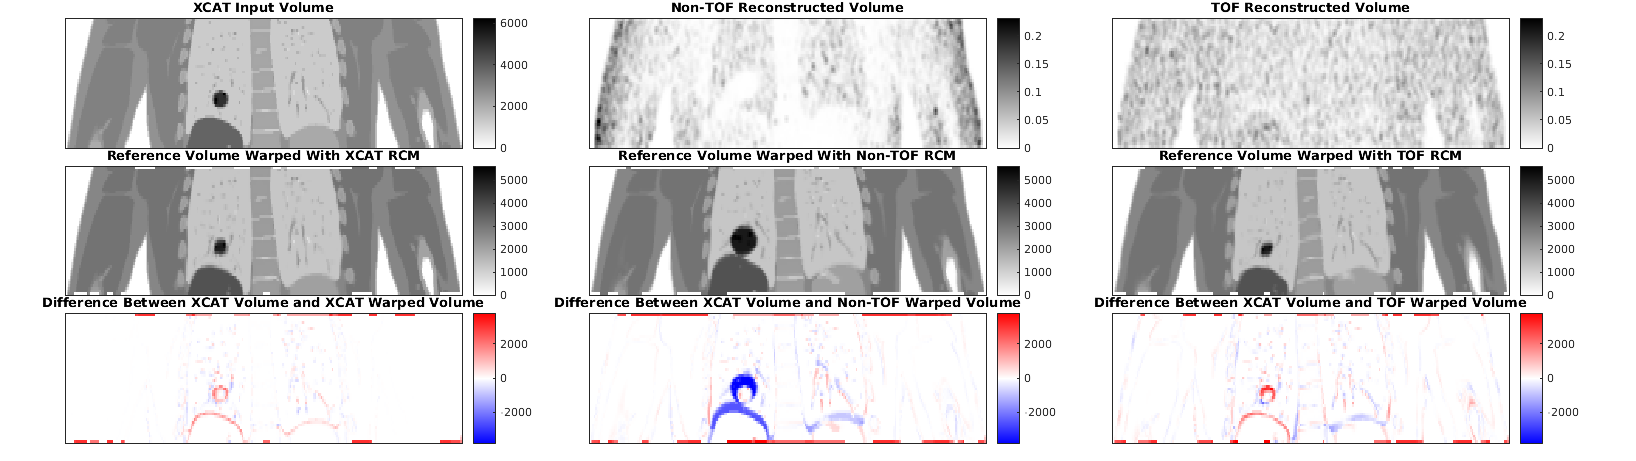
\includegraphics[width=1.0\linewidth]{figures/output.png}
                
                \captionsetup{singlelinecheck=false, justification=raggedright}
                \caption{All volumes correspond to end inhalation. First row from left to right: \gls{XCAT} \gls{PET} data, \gls{NAC} \gls{NTOF} reconstructed data and \gls{NAC} \gls{TOF} reconstructed data. Second row: \gls{RCM} applied to mean position \gls{XCAT} data with \gls{RCM} derived from \gls{XCAT} \gls{PET} data (left), \gls{NAC} \gls{NTOF} (middle) and \gls{NAC} \gls{TOF} (right) volumes. Colour map ranges are consistent for all images on this row. The third row from left to right: The difference between the estimated volumes from the second row with the \gls{XCAT} end-inhalation volume. Colour map ranges are consistent for all images on this row.} \label{fig:output}
            \end{figure*}
            
            \begin{table}
                \centering
                
                \captionsetup{singlelinecheck=false, justification=raggedright}
                \caption{Comparison of the \gls{MAPE} between the ground truth data and the volumes estimated from the \gls{XCAT} based \gls{RCM}, the volumes estimated from the \gls{NAC} \gls{NTOF} based \gls{RCM} and the volumes estimated from the \gls{NAC} \gls{TOF} based \gls{RCM}.}
                
                \resizebox*{1.0\linewidth}{!}
                {
                    \begin{tabular}{||c|ccc||}
                        \hline
                        \textbf{\gls{MAPE}} & \textbf{XCAT} & \textbf{\gls{NTOF}} & \textbf{\gls{TOF}} \\
                        \hline
                        \textbf{$1$} & $1.95$ & $8.35$ & $4.18$ \\
                        \textbf{$2$} & $1.59$ & $1.61$ & $1.84$ \\
                        \textbf{$3$} & $2.06$ & $9.91$ & $5.23$ \\
                        \textbf{$4$} & $1.97$ & $6.15$ & $3.68$ \\
                        \textbf{$5$} & $1.65$ & $4.45$ & $2.52$ \\
                        \textbf{$6$} & $1.95$ & $8.35$ & $4.18$ \\
                        \hline
                        \textbf{Mean} & $1.86$ & $6.47$ & $3.60$ \\
                        \hline
                    \end{tabular}
                } \label{tab:mape}
            \end{table}
            
            \begin{figure}
                \centering
                
                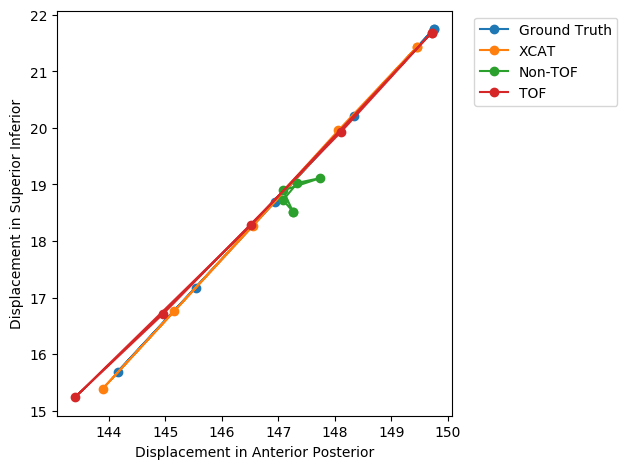
\includegraphics[width=1.0\linewidth]{figures/TOF.png}
                
                \captionsetup{singlelinecheck=false, justification=raggedright}
                \caption{The path of the \gls{COM} of the lesion. Horizontal (respectively vertical) axis corresponds to motion in the \gls{AP} (respectively \gls{SI}) direction over the six gates. Different curves denote \gls{COM} displacement for  ground truth data, the estimated data from the \gls{XCAT} based \gls{RCM}, the estimated data from the \gls{NAC} \gls{NTOF} based \gls{RCM} and the estimated data from the \gls{NAC} \gls{TOF} based \gls{RCM}.} \label{fig:com_graph}
            \end{figure}
            
             The reconstructed data, estimated volumes and difference can be seen in Figure~\ref{fig:output} and \gls{MAPE} are in Table~\ref{tab:mape}. The mean \gls{MAPE} was found to be lower for the \gls{NAC} \gls{TOF} data than for the \gls{NAC} \gls{NTOF}.
            
             \gls{COM} results can be seen in Figure~\ref{fig:com_graph}. The path of the \gls{NAC} \gls{TOF} data follows the ground truth path much closer than the \gls{NAC} \gls{NTOF} data, and is quite close to the gold standard \gls{XCAT}-derived motion.
            
        \subsection{Discussion and Conclusion} \label{impact_of_tof_on_respiratory_motion_modelling_using_nac_pet_discussion_and_conclusion}
            \gls{MM}s derived from \gls{NAC} \gls{TOF} volumes were found to be more robust than when using \gls{NAC} \gls{NTOF}, both visually and when comparing \gls{MAPE} and \gls{COM}. This was noticeable for the lung lesion in the thoracic cavity but also for other parts of the anatomy such as the liver. This is likely due to the improved image contrast of \gls{NAC} \gls{TOF} images.

            In the future, research will focus on investigating the robustness of the \gls{MM} estimation to different noise levels, acquisition duration and size of lesion.
    
    \longsection{Impact of TOF on Respiratory Motion Modelling using NAC PET: an Extension to Inter and Intra Respiratory Cycle Variation}{impact_of_tof_on_respiratory_motion_modelling_using_nac_pet_an_extension_to_inter_and_intra_respiratory_cycle_variation}
        \blindtext
        
        \subsection{Introduction} \label{impact_of_tof_on_respiratory_motion_modelling_using_nac_pet_an_extension_to_inter_and_intra_respiratory_cycle_variation_introduction}
        
        \subsection{Methods} \label{impact_of_tof_on_respiratory_motion_modelling_using_nac_pet_an_extension_to_inter_and_intra_respiratory_cycle_variation_methods}
            \blindtext
            
        \subsection{Results} \label{impact_of_tof_on_respiratory_motion_modelling_using_nac_pet_an_extension_to_inter_and_intra_respiratory_cycle_variation_results}
            \blindtext
            
        \subsection{Discussion and Conclusion} \label{impact_of_tof_on_respiratory_motion_modelling_using_nac_pet_an_extension_to_inter_and_intra_respiratory_cycle_variation_discussion_and_conclusion}
            \blindtext
    
    \longsection{Extension of Static PCA Based Data Driven Surrogate Signal Extraction to Dynamic PET}{extension_of_static_pca_based_data_driven_surrogate_signal_extraction_to_dynamic_pet}
        \blindtext
        
        \subsection{Introduction} \label{extension_of_static_pca_based_data_driven_surrogate_signal_extraction_to_dynamic_pet_introduction}
        
        \subsection{Methods} \label{extension_of_static_pca_based_data_driven_surrogate_signal_extraction_to_dynamic_pet_methods}
            \blindtext
            
        \subsection{Results} \label{extension_of_static_pca_based_data_driven_surrogate_signal_extraction_to_dynamic_pet_results}
            \blindtext
            
        \subsection{Discussion and Conclusion} \label{extension_of_static_pca_based_data_driven_surrogate_signal_extraction_to_dynamic_pet_discussion_and_conclusion}
            \blindtext
    
    \longsection{Feasibility of Neural Network Based Data Driven Surrogate Signal Extraction Methods for Dynamic PET}{feasibility_of_neural_network_based_data_driven_surrogate_signal_extraction_methods_for_dynamic_pet}
        \blindtext
        
        \subsection{Introduction} \label{feasibility_of_neural_network_based_data_driven_surrogate_signal_extraction_methods_for_dynamic_pet_introduction}
        
        \subsection{Methods} \label{feasibility_of_neural_network_based_data_driven_surrogate_signal_extraction_methods_for_dynamic_pet_methods}
            \blindtext
            
        \subsection{Results} \label{feasibility_of_neural_network_based_data_driven_surrogate_signal_extraction_methods_for_dynamic_pet_results}
            \blindtext
            
        \subsection{Discussion and Conclusion} \label{feasibility_of_neural_network_based_data_driven_surrogate_signal_extraction_methods_for_dynamic_pet_discussion_and_conclusion}
            \blindtext
